 	 \section{Introduction}
 	  
    
La modélisation par les processus dont les domaines d'application étaient relativement restreints à l'origine, n'a cessé de progresser. Elle s'impose, aujourd'hui, en tant qu'outil incontournable, placé au cœur de la gestion des organisations. La déclinaison des processus organisationnels au niveau des architectures logicielles a donné, entre autres, naissance au workflow afin de répondre à des besoins divers dont celui d'optimisation des processus opérationnels, support et de pilotage.

\section{Modélisation des processus workflow
}
La modélisation est une activité qui précède toute décision ou formulation, elle permet de représenter la description du système réel. Tout comme un système informatique, le système workflow comporte un certain nombre d'aspects à modéliser. Nous présentons en premier lieu ces aspects, nous décrivons en second lieu les principales techniques de modélisation utilisées dans le domaine de workflow et nous terminons cette section par évoquer certains aspects temporels et organisationnels des workflows.

\subsection{Aspects à modéliser}
\subsubsection{L'aspect fonctionnel}
L'aspect fonctionnel concerne l'identification des activités des processus que l'on souhaite modéliser. Il est important de comprendre qu'il ne s'agit pas uniquement d'identifier les fonctions des différents départements d'une organisation mais aussi de distinguer les activités composant un processus. La modélisation fonctionnelle doit également permettre d'établir la hiérarchie des activités, i.e. d'exprimer de possibles décompositions en termes de sous-processus. 

Enfin, le modèle fonctionnel doit aussi représenter le flux de données associées aux activités et les interdépendances de données entre les activités (data flow). 
\subsubsection{L'aspect comportemental}
L'aspect comportemental est un aspect primordial du workflow puisqu'il correspond à la dynamique du processus. Le comportement s'exprime par la modélisation d'un contrôle de flux entre les activités. Ce dernier permet d'indiquer la chronologie de l'exécution des activités, leur flux (séquentiel ou parallèle), les points de synchronisation entre activités ou au contraire, les points de disjonction. De plus, le modèle comportemental doit représenter les événements qui permettent de déclencher les activités. Nous soulignons l'importance de ce modèle, qui permet l'exécution du workflow. L'aspect comportemental est également appelé aspect de coordination.
\subsubsection{ L'aspect informationnel (données) }
Cet aspect concerne l'ensemble des informations et des données qui sont associées
aux activités. Le modèle informationnel, souvent négligé lors de l'implémentation d'un workflow \parencite{b3}, décrit en détail les relations qui existent entre les données, leur type et leur structure.
\subsubsection{L'aspect organisationnel }
Comme son nom l'indique, la partie organisationnelle concerne la description de l'organisation des acteurs de l'entreprise. Le modèle organisationnel peut soit refléter fidèlement l'organigramme de l'entreprise, c'est à dire la décomposition hiérarchique de celle-ci en départements et services soit décrire des unités organisationnelles dans lesquelles on identifie des acteurs. Selon la méthode choisie, la description est plus ou moins détaillée et permet d'établir des liens hiérarchiques entre les acteurs ainsi que des relations entre unités organisationnelles ou départements. Toutefois, quelle que soit la méthode retenue, la description des rôles associés aux différentes activités reste invariante. Les rôles créent l'interface entre le modèle organisationnel et les modèles représentant les activités.

\subsection{Techniques et outils de modélisation de workflow}

Associés aux aspects à modéliser définis précédemment, un certain nombre d'outils de modélisation peuvent être employés pour décrire le comportement des flux de travail.

\subsubsection{Réseaux de Petri et workflow
}
Les Réseaux de Petri (RdPs) \parencite{RdPs} constituent un formalisme majeur pour modéliser les processus workflows. Une des forces des RdPs est la base mathématique forte qu'ils offrent avec une représentation graphique. Dans cette section, nous résumons la projection topographique entre concepts de workflow et de RdP .%[1, 11, 65]. 

Un processus définit les tâches aussi bien que les conditions pour leur exécution. En utilisant les RdPs, un processus est représenté en conversant sa seule entrée (i.e., un nœud du début) dans une place sans arcs entrants, et sa seule sortie (i.e., nœud de la fin) dans une place sans arcs sortants. Les conditions sont représentées par des places, et les tâches par des transitions. Habituellement, un processus spécifié par RdP devrait accomplir deux exigences : (1) il doit être possible d'accéder à tout moment un état pour lequel il y a un jeton dans la place finale, et (2) quand il y a un jeton dans la place finale, tous les autres jetons auraient dû disparaître.

Dans un processus modélisé par un RdP, une transition active correspond à un workitem, et le tir d'une transition à une instance de l'activité. Certains work-items peuvent seulement être transformés dans une instance d'activité une fois ils sont déclenchés. Un déclencheur pourrait correspondre à une initiative du participant, à un événement externe ou à un signal du temps initié par l'environnement. A chaque transition correspondante à une tâche qui exige un déclencheur, une autre place d'entrée est ajoutée. Une occurrence du déclencheur apporte un jeton dans cette place supplémentaire. Le jeton est consommé une fois la transition appropriée est franchie. Un échec pendant l'exécution d'une tâche exige un 'rollback' (i.e., revenir à l'état antérieur au début de l'activité). Quand une activité sera complétée avec succès, des changements deviennent définitifs.

\subsubsection{UML et workflow}


Les diagrammes d'états/transitions sont un autre formalisme majeur pour la modélisation des processus workflows. Ils ont été inventés par Harel \parencite{Harel}, et ont été incorporés dans UML (Unified Modelling Language)  \parencite{UML}, dans une forme légèrement différente. Weissenfels et al. \parencite{EDBT'98} ont investi sur l'usage des diagrammes d'états/transitions pour modéliser les processus workflows (le projet Mentor WfMS). Nous pouvons aussi citer Blake \parencite{WETICE'02} qui a présenté une approche systématique pour la modélisation des workflows en utilisant UML (le projet WARP). 

Dans le projet Mentor WfMS \parencite{EDBT'98}, les activités reflètent la décomposition fonctionnelle d'un système et dénotent les composants actifs d'une spécification; elles correspondent directement aux activités d'un workflow. Un diagramme d'activités spécifie le flot de données entre les activités, dans la forme d'un graphe orienté avec les éléments de données comme annotations des arcs. Les diagrammes d'états capturent le comportement d'un système en spécifiant le flot de contrôle entre les activités.

Pour le projet WARP (Workflow Automation through Agent-based Reflective Processes) \parencite{WETICE'02}, l'approche utilisée distingue entre les vues structurelles, fonctionnelles, non fonctionnelles, et opérationnelles. Les vues structurelles informe sur les activités, la définition des rôles, et la composition du workflow. Elles sont représentées dans UML par les diagrammes des classes. Les vues fonctionnelles montrent le flot de données et de contrôle du workflow en utilisant les diagrammes d'activités UML. Les vues non-fonctionnelles (traitement des erreurs, concurrence, atomicité, etc.) utilisent le flot de données et de contrôle et peuvent être modélisées aussi par les diagrammes d'activités. Finalement, les vues opérationnelles sont reliées à l'initiation des instances du workflow, et la coordination pour l'achèvement du workflow. Ces vues peuvent être modélisées par les diagrammes de séquence UML.

\subsubsection{YAWL}
YAWL (Yet Another Workflow Language) [2] est basé sur les RdPs avec des caractéristiques additionnelles pour faciliter la modélisation des workflows complexes. YAWL hérite de la classe des RdPs et s'étend par la modélisation de l'instance multiple, les tâches composites, le retrait des jetons et les transitions connectées directement.

La spécification du workflow dans YAWL est une sorte de réseaux de workflow étendu (EWF-nets) qui forme une hiérarchie. Une tâche est soit atomique soit composite. Chaque tâche composite fait référence à un unique EWF-net dans le niveau le plus bas de la hiérarchie. Les tâches atomiques forment les feuilles de l'arbre. Il y a un seul EWF-net non référencé par une tâche composite. Cet EWF-net est nommée le niveau le plus haut du workflow et forme la racine. 

Chaque EWF-net consiste en des tâches (composites ou atomiques) et des conditions qui peuvent être interprétées comme des places. 
Chaque EWF-net a une unique condition d'entrée et une unique condition de sortie. Contrairement aux RdPs, il est possible de connecter les transitions. Sémantiquement, cette construction peut être interprétée comme une condition ignorée.

Chaque tâche peut avoir des instances multiples. Nous pouvons créer un seuil maximal et un seuil minimal pour le nombre d'instances après l'initiation d'une tâche. En plus, il est possible d'indiquer que la tâche se termine au moment ou certaines instances seuils sont achevées

\section{Les réseaux de Petri}

Les réseaux de Petri(Petri,1962)sont une généralisation des automates a états. Ils offrent un contexte général pour modéliser la concurrence et la synchronisation dans les systèmes distribués. Un réseau de Petri est un graphe biparti alterné qui possède deux types de nœuds: les places(cercles)et les transitions(rectangles). Des arcs(flèches) relient les places aux transitions(figure \ref{fig:2 rdp}). L'état du système,nommé marquage,est défini par la répartition des jetons dans les places. Une transition est franchissable sous certaines conditions, notamment lorsqu'il y a suffisamment de jetons dans ses places d’entrée. Le franchissement d’une transition se traduit par une modification du marquage consistant en la consommation des jetons indispensables au franchissement de la transition et la création éventuelle de nouveaux jetons dans les places en sortie de la transition.
\begin{figure}[h]
	\centering
	
	\begin{subfigure}[b]{0.3\textwidth}
		\centering
		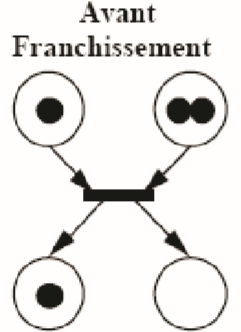
\includegraphics[width=\textwidth]{petrif1}
		\caption{$M_{t}=(1,2,1,0)$}
		\label{fig:three sin x}
	\end{subfigure}
	\hfill
	\begin{subfigure}[b]{0.3\textwidth}
		\centering
		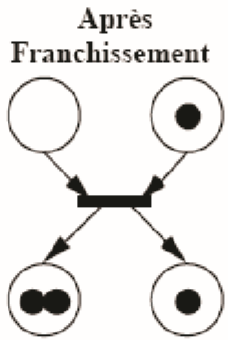
\includegraphics[width=\textwidth]{pitrif2}
		\caption{$M_{t+1}=(0,1,2,1)$}
		\label{fig:five over x}
	\end{subfigure}
	
	\caption{Opération de franchissement}
	\label{fig:2 rdp}
\end{figure}

\subsection{Définition}

\begin{defn}\textbf{\textbf{(Réseau de Petri simple):}}
	\\
Un réseau de Petri simple est un tuple
 (P,T,Pre,Post,M0):
 
 \begin{itemize}
\item  	P est un ensemble final de places,
\item T est un ensemble final de transition $ (P \cap T = \theta ) $ ,
\item Pre: $P \times T \to N$ est la fonction d'incidence avant,
\item Post: $P \times T \to N$ est la fonction d'incidence arriére,
\item $M_{0}$ et le marquage initial $M_{0}:  P \to N$.
  \end{itemize}

\end{defn}




Un réseau de Petri peut-être evucommeun système de transitions dont les états sont les marquages du réseau et les transitions entre états correspondent au franchissement des transitions du réseau.
\subsubsection{Propriétés des réseaux de Petri}
il existe un certain nombre de propriétés qui ont été définis pour les réseaux de Petri, à savoir, le caractère borné, la réinitilisation la vivacité , la conservation, la terminaison (Diaz, 2001). Certaines de ces propriétés sont dites propriétés dynamiques car elles dépendent du marquage initial et sont liées à l'évolution du réseau,alors que d'autres sont dites propriétés statiques du fait qu'elles soient liées à la typologie du réseau et indépendantes du marquage initial.


\begin{defn}\textbf{\textbf{(Réseau de Petri borné):}}\\
Une place $ P_{i} $ est bornée pour un marquage initial $ M_{0} $ si pour tout marquage accessible à partir de $ M_{0} $, le nombre de jetons dans Pi reste borné. Elle est dite k-bornée si le nombre de jetons dans $ P_{i} $ est toujours inférieur ou égal à k. Un RdP est(k) borné si tout esses places sont(k)bornées.

\end{defn}

\begin{exmp}
 Un RdP peut ne pas être borné. Sur l'exemple représenté à la (figure \ref{fig:rdpborn}), la transition $ T_{1} $ admet la place $ P_{1} $ comme unique place d'entrée.La place P1 a un jeton:la transition $ T_{1} $
\end{exmp}

\begin{figure}[h]
	\centering
	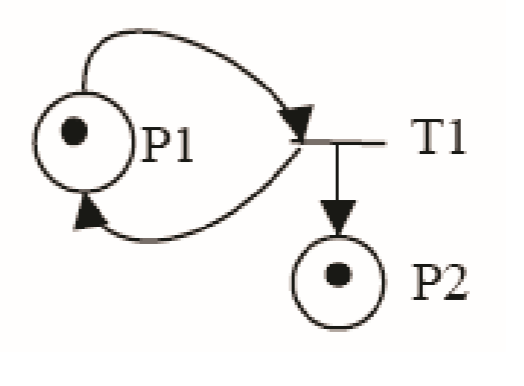
\includegraphics[width=0.5\linewidth]{images/Rdpborn}
	\caption{Réseau de Petri non borné}
	\label{fig:rdpborn}
\end{figure}

est franchissable. Comme $ P_{1} $ est aussi place de sortie de $ T_{1} $,le franchissement de $ T_{1} $ ne change pas le marquage de $ P_{1} $.La transition $ T_{1} $ est donc franchissable en permanence et peut donc être franchie un nombre de fois infini.Chaque franchissement de $ T_{1} $ ajoute un jeton dans $ P_{2} $ dont le marquage va donc tendre vers l'infini.

\begin{defn}\textbf{Réseau de Petri sauf:}\\
	Un RdP est sauf ou binaire pour un marquage initial M0 s'il est un borné.
 
\end{defn}


\begin{defn}\textbf{La vivacité:}\\
	Une transition $ T_{j} $ est vivante pour un marquage initial $ M_{0} $ si pour tout marquage accessible $ M_{k} $ , il existe une séquence de franchissement $ S $ à partir de $ M_{k} $ contenant $T_{j}: M_{k} \in^{*} M_{0},   \exists S,M_{k}| S>$ et $S = ... T_{j} ...$
	\\
	
	Si une transition $ T_{j} $ est vivante alors, à tout instant, on sait que $ T_{j} $ peut être franchie dans le futur. Dans le cas d'un réseau de Petri modélisant un système fonctionnant en permanence, si une transition n'est pas vivante et si une fonction du système est associée au franchissement de cette transition,ce la veut dire qu'à partir d’un certain instant ,cette fonction ne sera plus disponible dans le futur, ce qui peut traduire une erreur ou une panne.
	
\end{defn}



\begin{defn}\textbf{Blocage:}\\
	Un blocage (ou état puits)est un marquage pour lequel aucune transition n'est validée.
\end{defn}


Un réseau de Petri est dit sans blocage pour un marquage initial M0 si aucun marquage accessible n'est un blocage.
\begin{figure}[h]
	\centering
	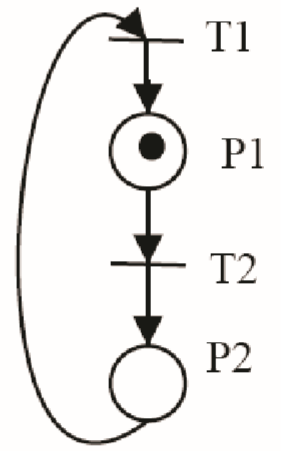
\includegraphics[width=0.2\linewidth]{images/Petrivivant}
	\caption{Réseau de Petri vivant}
	\label{fig:petrivivant}
\end{figure}
\begin{figure}[h]
	\centering
	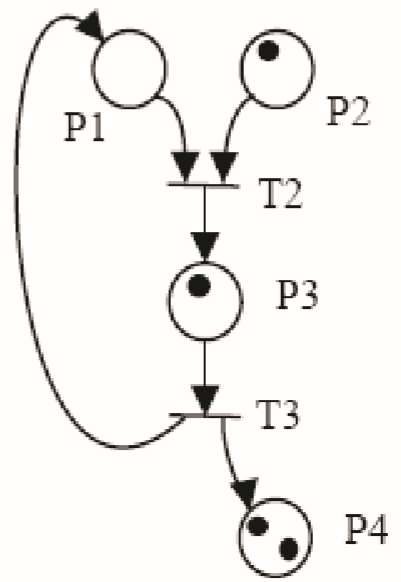
\includegraphics[width=0.25\linewidth]{images/Petribloquant}
	\caption{Exemple de réseau de Petri bloquant}
	\label{fig:petribloquant}
\end{figure}

Le réseau de Petri de la (Figure 3.7), par exemple ,a pour blocage le marquage: 
M = (1,0,0,1).

\begin{defn} \textbf{(états d' accueil et Réseau de Petri réinitialisable ) }\\
Un RdP a un état d’accueil $ M_{a} $ pour un marquage initial $ M_{0} $ si pour tout marquage accessible $ M_{k} $ à partir de $ M_{0} $, il existe une séquence de franchissement permettant d'atteindre le marquage
 $M_{a}: \forall M_{k} \in^{*} M_{0},   \exists S_{j},M_{k}|S_{j}>M_{a}$
\end{defn}
Un RdP est réinitialisable pour un marquage initial $ M_{0} $ si $ M_{0} $ est un\\
 état d'accueil.
\\

Si un réseau de Petri présente un état d’accueil, il est facile de vérifier s’il est sans blocage et d'étudier sa vivacité.


\subsubsection{Les réseaux de Petri colorés}
Les réseaux colorés(Jensen, 1997)ont été introduits afin de modéliser des systèmes complexes tout en gardant les possibilités de vérification. Lorsque le nombre d'entités du système à modéliser est important,la taille du réseau de Petri devient rapidement énorme,et si les entités présentent des comportements similaires, l'usage des réseaux colorés permet de condenser le modèle. En effet, une couleur est une information attachée à un jeton. Cette information permet de distinguer des jetons entre eux et peut être de type quelconque. Par conséquent, une place peut contenir des jetons de différentes couleurs et une transition peut être franchie de différentes manières, selon la couleur. Ceci est réalisé en attachant un domaine de couleur à chaque place et à chaque transition. Ainsi, les arcs ne sont pas seulement étiquetés par le nombre de jetons mais aussi par leurs couleurs.Le franchissement d'une transition est alors conditionné par la présence dans les places en entrée du nombre de jetons nécessaires, qui en plus satisfont les couleurs qui étiquettent les arcs. Après le franchissement d'une transition,les jetons qui étiquettent les arcs d'entrée sont retirés des places en entrée tandis que ceux qui étiquettent les arcs de sortie sont ajoutés aux places en sortie de cette transition.

Ainsi,pour un même système,le nombre de comportements qui peuvent être exprimés par un réseau coloré est nettement plus élevé qu’avec un réseau simple. Ce sont des réseaux très adaptés aux architectures distribuées.D'autant plus qu`a tout réseau coloré correspond un réseau de Petri simple qui lui est isomorphe.Ce ci permet donc d'exploiter les mêmes techniques d'analyse que celles développées pour les réseaux simples en plus d'autres qui ont été complétées et adaptées aux réseaux colorés telle que le support de la
 hiérarchisation.

\begin{defn}\textbf{Réseau de Petri Colorés:}\\
	Un réseau de Petri Coloré (CPN) et un tuple $(\bigtriangleup,P,T,Arc,Noeud,Couleur,Grade,E,M_{0}) $ où :
 

\end{defn}


\begin{itemize}
\item\textbf{ $\bigtriangleup$:}  est un ensemble de domaines de couleurs (chaque domaine est un ensemble fini et non vide ).
\item \textbf{$ Arc $:} est un ensemble fini d'arcs tel que $P \cap Arc = T \cap Arc = \emptyset $
\item \textbf{$Nœud$}:  est la fonction $Nœud$ ,$Nœud$ : $Arc \longrightarrow	P \times T \cup T \times P $.

\item   \textbf{$ Couleur $} : $P \longrightarrow PowerSet(\bigtriangleup)$. $Couleur(p)$ est la fonction couleur qui associe à chaque place un domaine de couleur.

\item \textbf{$ Garde $}: est une garde, qui fait correspondre à chaque transition une expression booléenne.Les variables de la garde appartiennent à $\bigtriangleup$.
\item \textbf{$ E $}: est l'application qui associe à chaque arc, un élément de Couleur(p)MS où p est une place appartenant à l'arc. E indique le nombre de jetons colorés à recevoir de la place qui se trouve en entrée de la transition,et le nombre de ceux à produire dans la place qui se trouve en sortie. 

\item \textbf{$ M_{0} $}: est l'application qui associe à chaque place p,un élément de Couleur(p) $ M_{S} $. $ M_{0}$ (p)indique la distribution initia le des jetons colorés dans la place p.

\end{itemize}
 
 
 
De maniéré générale,un marquage M d’un réseau coloré est une application qui associe à chaque place p, un élément de Couleur(p)MS. M(p) est un multi-ensemble sur Couleur(p)qui indique les marques colorées présentes dans la place p au marquage M. L'état du modèle est défini par un marquage coloré.


\section{Modélisation Des Politiques De Sécurité}

Durant les dernières années, l'utilisation des réseaux de Petri s'est répandue grâce au nombre de travaux qui a été développé pour enrichir les réseaux de Petri ainsi que la disponibilité des outils. Selon de nombreux chercheurs (Osborn, 2002), les réseaux de Petri sont le seul formalisme qui permet de modéliser la structure du système et de faire des analyses qualitative et quantitative. Les réseaux de Petri ont été utilisés pour la vérification de la sécurité(Ahmed and Tripathi,2003),pour la spécification des autorisations dans les workflows \parencite{ESORICS'96},l'analyse des politiques de sécurité y compris les politiques de contrôle d'accès discrétionnaires (Kumaretal. ,2002; Knorr, 2000), mandataires(Knorr, 2001; Varadharajan, 1991; Juopperi, 1995; Juszczyszyn, 2003; Jiangetal., 2004; Rakkay and Boucheneb, 2006; Zhangetal., 2006b; Zhangetal., 2006a) et à base de ro les(Koch et al.,2002;Rakkay and Boucheneb, 2007;Shafiq et al.,2005).














